\documentclass{article} % For LaTeX2e
\usepackage{iclr2018_conference,times}
\usepackage{hyperref}
\usepackage{url}
\usepackage{graphicx}


\title{(tentative) Learning Neural Markers of Schizophrenia Disorder Using Recurrent Neural Networks}

% Authors must not appear in the submitted version. They should be hidden
% as long as the \iclrfinalcopy macro remains commented out below.
% Non-anonymous submissions will be rejected without review.

\author{Antiquus S.~Hippocampus, Natalia Cerebro \& Amelie P. Amygdale \thanks{ Use footnote for providing further information
about author (webpage, alternative address)---\emph{not} for acknowledging
funding agencies.  Funding acknowledgements go at the end of the paper.} \\
Department of Computer Science\\
Cranberry-Lemon University\\
Pittsburgh, PA 15213, USA \\
\texttt{\{hippo,brain,jen\}@cs.cranberry-lemon.edu} \\
\And
Ji Q. Ren \& Yevgeny LeNet \\
Department of Computational Neuroscience \\
University of the Witwatersrand \\
Joburg, South Africa \\
\texttt{\{robot,net\}@wits.ac.za} \\
\AND
Coauthor \\
Affiliation \\
Address \\
\texttt{email}
}

% The \author macro works with any number of authors. There are two commands
% used to separate the names and addresses of multiple authors: \And and \AND.
%
% Using \And between authors leaves it to \LaTeX{} to determine where to break
% the lines. Using \AND forces a linebreak at that point. So, if \LaTeX{}
% puts 3 of 4 authors names on the first line, and the last on the second
% line, try using \AND instead of \And before the third author name.

\newcommand{\fix}{\marginpar{FIX}}
\newcommand{\new}{\marginpar{NEW}}

%\iclrfinalcopy % Uncomment for camera-ready version, but NOT for submission.

\begin{document}


\maketitle

% Outline: 
% 1. Introduction: RNNs and CNNs being used for variety of recognition and diagnosis tasks. Problem with previous attempts
% to learn features from brain imaging data (fmri). High variability in brain responses across individuals.
% 2. Related Work: previous work on frmi, previous work to learn from videos, previous work to diagnose schizophrenia 
% 4. Methods
%   4.1 dataset
%   4.2 recurrent-convolutional neural nets for feature learning from fmri segments
% 5. Experiments: 
%   5.1 effectiveness of RNNs and R-CNNs to learn discriminative features from fmri
%	  5.2 generalizability of learned features across datasets
% 6. Discussion
% 7. Conclusion

\begin{abstract}
... Here we propose a new method based on recurrent-convolutional neural networks to automatically learn useful representations from short segments of fMRI recordings...
\end{abstract}

\section{Methods}

\subsection{Dataset}
One scane was captured every 2 seconds. Each session (??) consists of a single fMRI scanning session which lasted for almost 5 minutes (??). Data from each session was split to windows of 32 or 128 seconds which formed the samples used for training, evaluation, and test.  

\subsection{Recurrent-Convolutional Neural Networks}
We used recurrent-convolutional nerual networks (R-CNN) to learn discriminative features for the problem of distinguishing normal and schizophrenic individuals. We tried several different architectures consisting of RNNs as well as R-CNNs. The input to the network is a 3-dimensional tensor (3D brain scans). We used 3-dimensional convolutions followed by max-pooling to extract position and scale independent features that would generalize across individuals. 

Long Short-Term Memory (LSTM) network was used to model the temporal structure of data within each sample. LSTMs are known for their ability in learning long-term dependencies between inputs. 
To implement the R-CNN, we constructed identical convolutional networks for each time frame with weights shared among all of them. Outputs of each CNN was then reshaped into a vector which was fed as input to the LSTM network at each time step. Figure-\ref{fig1} shows an overview of the recurrent-convolutional network used here. 
We used Adam optimizer with default parameter values ($\beta_1=0.9, \beta_2=0.999, \epsilon=10^{-8}$). 
10-fold cross-validation was used to evaluate the performance for each proposed model. $l_2$ regularizer was used on all convolutional and fully connected weights. 
3D-convolutions of size $3\times3\times3$ with stride 1 were used. Each block of convolutions were followed by a maxpool layer of size 2 and stride 2. Feature map size was dividing by 2 after each maxpool layer. Size of the input to the network was $(53\times64\times37)$.

A different subset of subjects were assigned to the test set for each fold and data from the rest of the subjects were used for training and validation (without overlap between train and validation sets). For training, samples within each batch were generated by randomly selecting time windows from different subjects. All possible time windows of size $T$ from all subjects were used for training, validation and test. For each fold training was done for 10 folds. We used the validation set to for early stopping of training. After each training epoch, performance on the validation set was computed. Training was performed for 10 epochs and test performance was computed for the network state with highest validation score. 

We used a batch size of 64 for all models. Larger convolutional models were trained using synchronous gradient descent on 16 GPUs. 

\begin{figure}[t]
\begin{center}
\label{fig1}
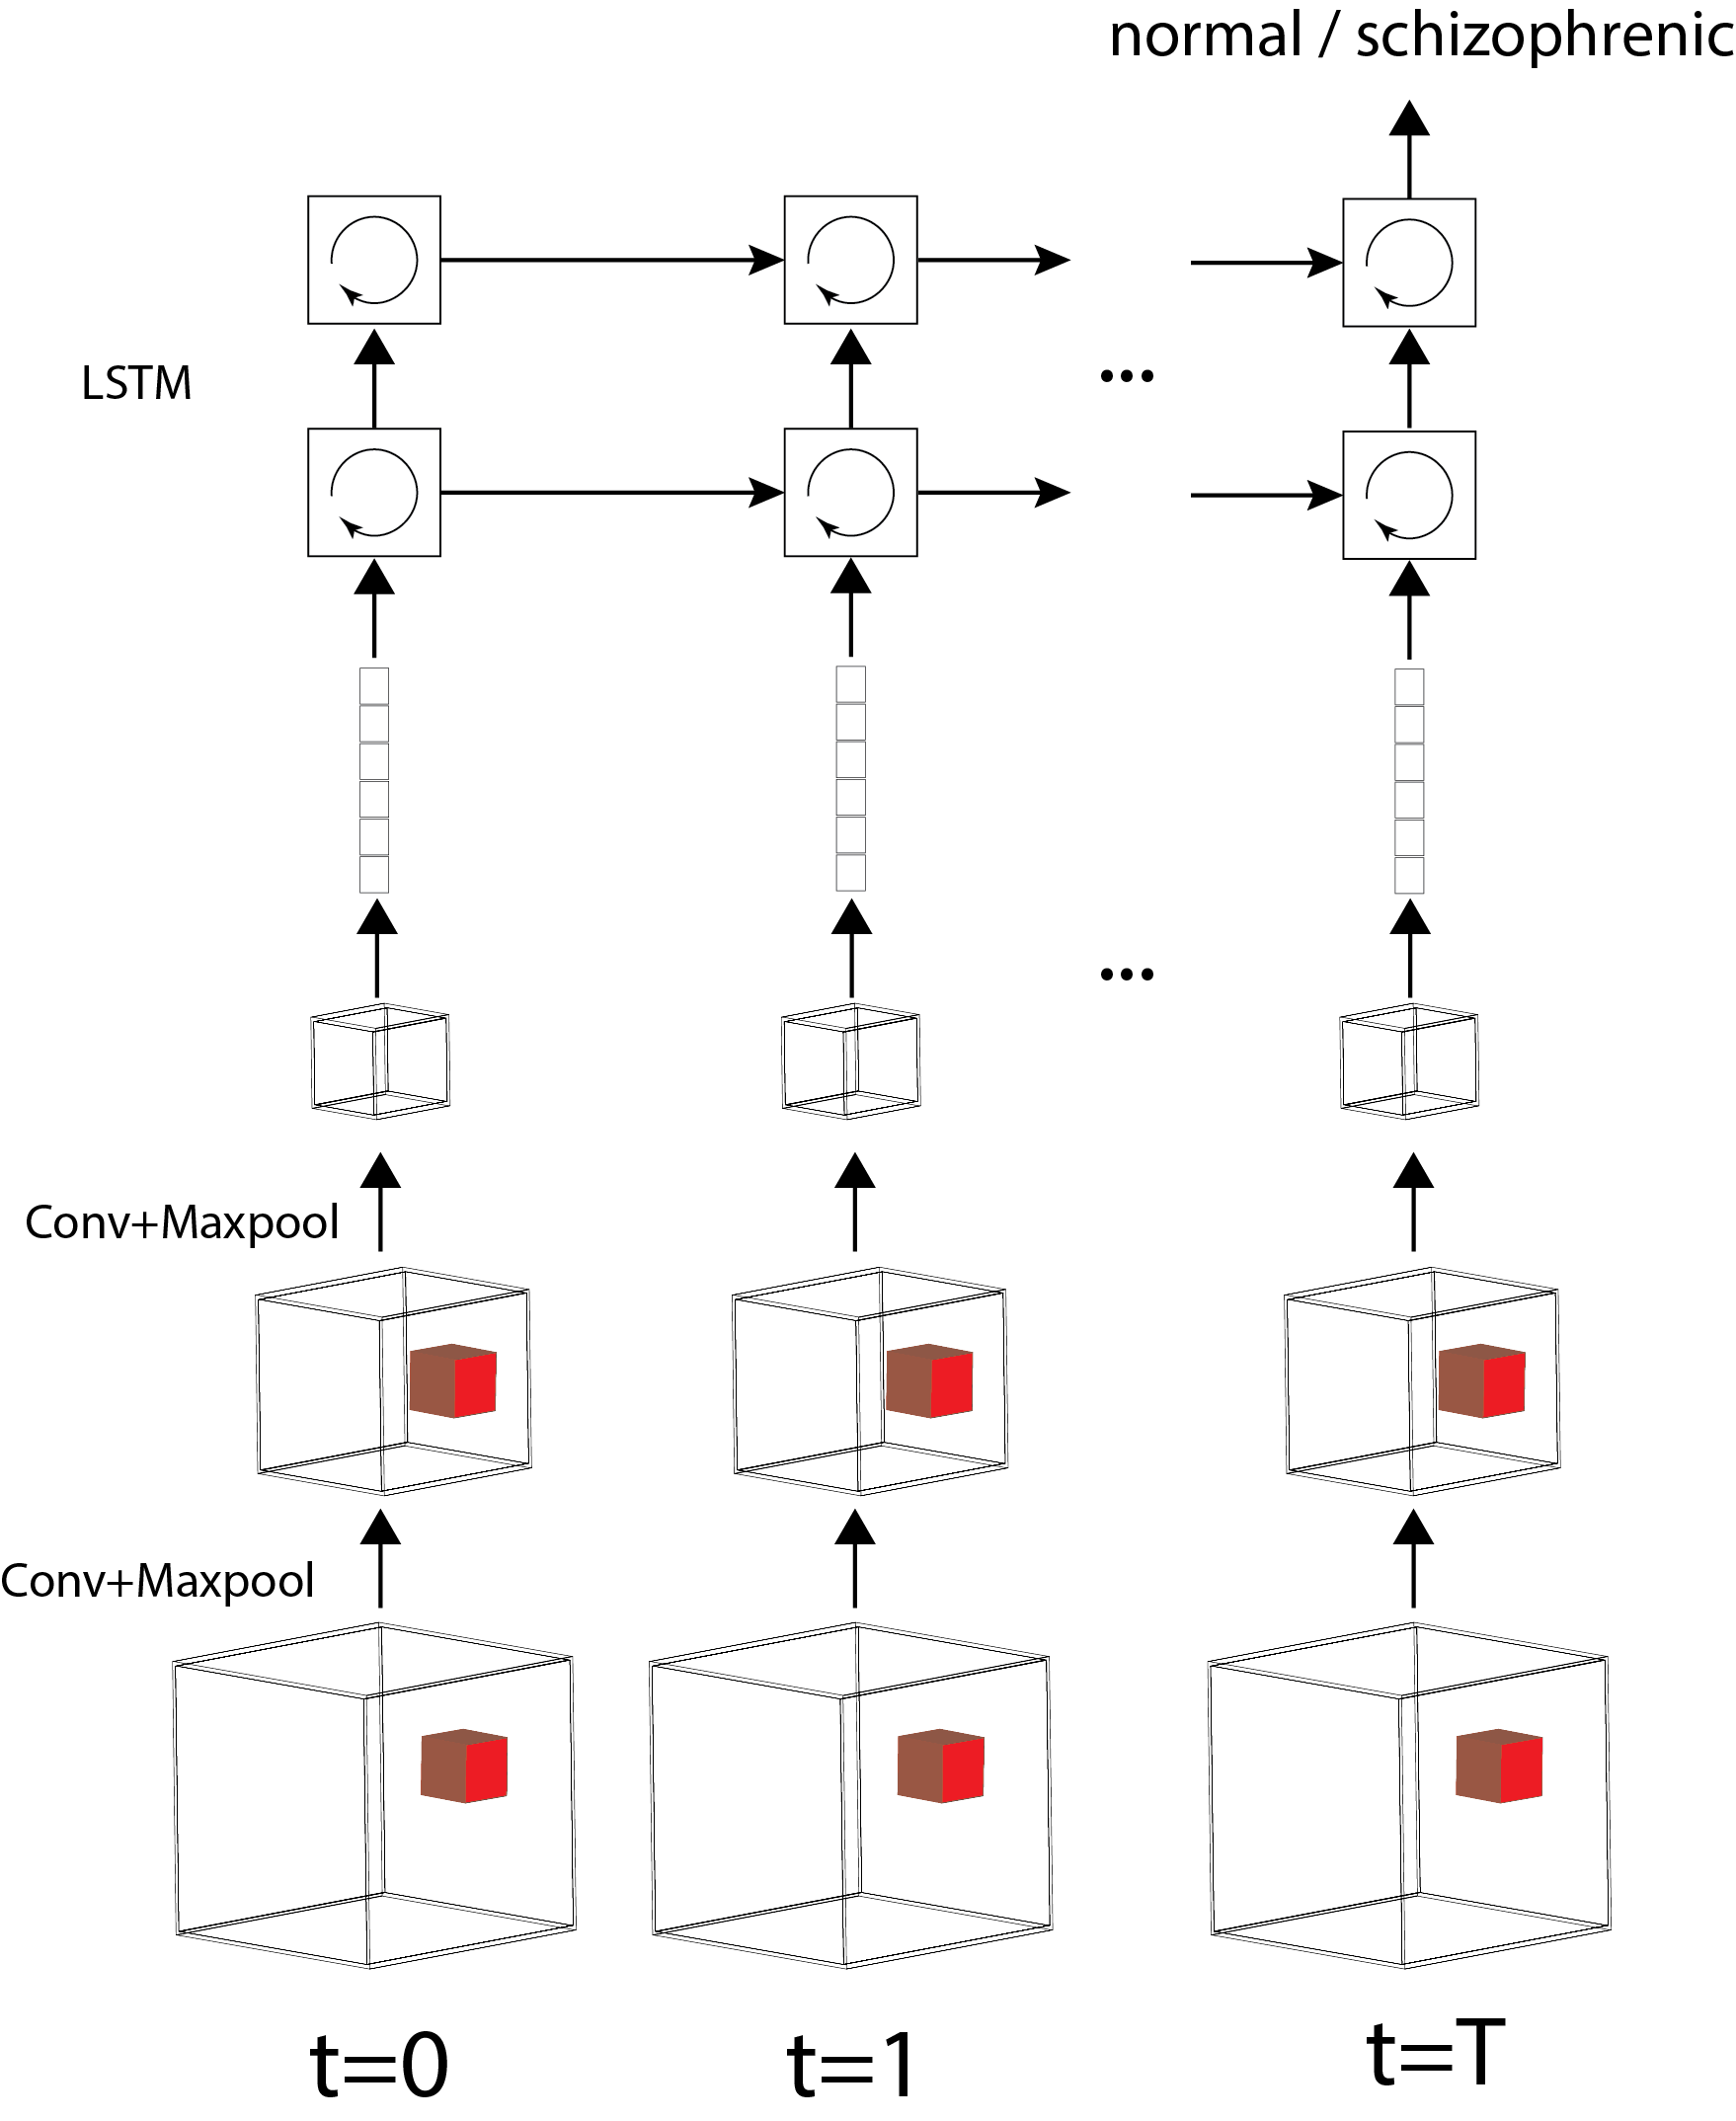
\includegraphics[width=3in]{figures/overview.png}
%\framebox[4.0in]{$\;$}
\end{center}
\caption{Overview of the method used.}
\end{figure}

\subsection{Data Preprocessing}


\subsubsection*{Acknowledgments}

Use unnumbered third level headings for the acknowledgments. All
acknowledgments, including those to funding agencies, go at the end of the paper.

\bibliography{iclr2018_conference}
\bibliographystyle{iclr2018_conference}

\end{document}
